\begin{definition}[Relative Monicity~\cite{endrullis2024generalized}]
    \label{def:relative_monicity}
    Let $A,B,C$ and $X$ be objects, $\Gamma$ a set of objects, $S$ a set of morphisms to $A$ and $u:C\to A$ a morphism. A morphism $f : A \to B$ is called 
    \begin{enumerate}[label=(\roman*)] 
        \item 
            \emph{monic for $S$} 
            if $g \star f = h \star f$ implies $g = h$ for all $g, h \in S$;
        \item 
            \emph{$X$-monic} if $f$ is monic for $\operatorname{Hom}(X, A)$.
        \item \emph{$X$-monic outside of $u$}, if $f$ is monic for \( \operatorname{Hom}(X,A) \setminus \left ( \operatorname{Hom}(X,C) \star u \right ) \).
        \item  \emph{$\Gamma$-monic} if $f$ is $X$-monic for every $X \in \Gamma$.
    \end{enumerate}
\end{definition} 
The concepts defined above are restricted versions of the concept of monicity.
\begin{example}[Edge-Monicity \cite{endrullis2024generalized_lmcs}]
    In $\mathbf{Graph}$, let 
    $\Gamma = \left\{ \vcenter{\hbox{
    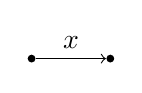
\begin{tikzpicture}[baseline=-0.5ex]
    \node[circle, fill, inner sep=1pt] (A) at (0,0) {};
    \node[circle, fill, inner sep=1pt] (B) at (1,0) {};
    \draw[->] (A) -- (B) node[midway, above] {$x$};
    \end{tikzpicture}
    }} \mid x \text{ is an edge label} \right\}$.
    
    A morphism $f : G \to H$ that does not identify edges (but may identify nodes) is not necessarily monic, but it is $\Gamma$-monic. In this particular case for $\mathbf{Graph}$, we will say that $f$ is \textbf{edge-monic}.
\end{example}